\chapter[Resultados]{Resultados}
\label{result}

	Para cada \textit{shader} foram plotados os gráficos para as métricas relacionadas ao vértice e ao fragmento. Após as plotagens, percebeu-se que todos os gráficos de todos os \textit{shaders} relacionados ao vértice deram uma função linear (diferindo na inclinação) e os relacionados ao fragmento deram uma curva de formato semelhante. A Figura \ref{plotred} e a Figura \ref{plotrefl} mostram os gráficos plotados, com relação ao \textit{vertex} e \textit{fragment shaders} de cada \textit{shader} implementado, que demonstram a semelhança destas curvas.

	 Os ajustes em relação às curvas pré-definidas (linear, exponencial, segundo e terceiro graus) também foram calculados e plotados (Figura \ref{linear} referente ao \textit{Reflection Shader}). Também foram determinados os menores erros associados, a fim de descobrir qual a curva melhor ajustava as medições do \textit{fragment shader}. Pela a análise do menor erro, calculado de acordo com a Seção \ref{metminqua}, todos os \textit{shaders} se aproximaram melhor de uma curva de segundo grau. Estes ajustes também foram feitos para as curvas obtidas do tempo do processo de renderização \textit{versus} a quantidade de polígonos (que foi discutido na Seção \ref{gpu}). A análise do menor erro calculado indicou que, assim como o \textit{fragment shader}, todas as curvas se aproximaram melhor de uma curva de segundo grau.

	As equações calculadas para cada \textit{shader} (relacionadas ao vértice e fragmento) são mostradas na Tabela \ref{equacoes}. Embora as curvas sejam de mesma família, os seus coeficientes não são. Os \textit{shaders} relativamente mais simples tem inclinação de reta menor, assim como o coeficiente do termo $x^2$. Pela análise das equações, é possível perceber que o \textit{vertex shader} de melhor desempenho é o do \textit{Flat Shader}, que apenas determina as coordenadas $x$ e $y$, já que o $z$ é sempre zero. O de pior desempenho é o \textit{Gouraud Shader}, que faz os cálculos de luz por vértice. Já o \textit{fragment shader} de melhor desempenho é o do \textit{Red Shader}, que apenas determina que a cor do fragmento seja vermelha. O de pior desempenho foi o do \textit{Phong Shader}, que faz os cálculos de luz por fragmento.

	Outra observação que pode ser feita é quanto aos \textit{shaders Gouraud} e \textit{Phong}, pois eles realizam o mesmo cálculo, porém o primeiro faz no \textit{vertex shader} e o segundo, no \textit{fragment shader}. Pela análise das equações, o desempenho relacionado ao \textit{vertex shader} do \textit{Gouraud} é pior que a do \textit{Phong} e a relacionado ao \textit{fragment shader} é melhor.  Além disso, com as equações é possível estimar a quantidade de instruções por segundo por vértice ou por fragmento. Tomando como exemplo o \textit{Toon Shader}, que sua equação para o \textit{vertex shader} é  $y = 10.17 \times 10^6 + 4673.96t$, o número de instruções por segundo por vértice estimado para 60000 polígonos é de $29.06 \times 10^7$. Realizando a medição com a ferramenta \textit{Adreno Profiler} foi possível perceber que este valor é próximo ao medido, que foi $28.49 \times 10^7$.

	As equações relacionadas a todo o processo de renderização também foram calculadas e podem ser vistas na Tabela \ref{eqrender}. Assim como no caso anterior, elas são da mesma família mas possuem coeficientes diferentes. De acordo com estas equações, o \textit{shader} de pior desempenho é o de Reflexão, que pela análise anterior, os \textit{shaders} de vértice e fragmento eram uns dos de pior desempenho. Outro resultado relevante é quanto ao \textit{Gouraud} e \textit{Phong shaders}, em que na análise anterior, o primeiro possui o pior desempenho entre os \textit{shaders} de vértice e o segundo, entre os \textit{shaders} de fragmento.  Mas o que possui o pior desempenho entre os dois, em relação ao processo de renderização como um todo, é o \textit{Phong shader}. Este resultado é consistente, pois o \textit{fragment shader}, pelo experimento realizado, possui complexidade algorítimica $n^2$ e o \textit{vertex shader}, $n$, influenciando neste pior desempenho. 	Pelo experimento realizado, os \textit{shaders} de melhores desempenhos são o \textit{Flat}, \textit{Toon} e \textit{Red}. Além disso, utilizando as equações calculadas, a fim de estimar o tempo para 200000 polígonos, por exemplo, essa análise se confirma, como é mostrada na Tabela \ref{estimativa}.
	
	Assim, o processo utilizado neste trabalho de estimação da complexidade algorítimica calculada de forma empírica, pode ser resumido na Figura \ref{processo}. A etapa de Implementar \textit{Shaders} pode ser feita por meio da utilização da base do projeto implementado, extendendo-se da classe \textit{Shader} e implementando os métodos abstratos, como explicado na Seção \ref{imp}. A etapa Realização das Medições é feita de forma manual, dependendo do \textit{profiler} de GPU adequado para o \textit{device} utilizado. E a etapa Plotar Gráficos, Ajustar Curvas e Obter Equações pode ser feita através do \textit{script} criado para o ajuste das curvas.

	\begin{table}[ht]
	\centering	
	\begin{tabularx}{0.9\textwidth}{cXX}
		\toprule
		\textbf{Nome} & \textbf{Instruções por Segundo por Vértice} & \textbf{Instruções por Segundo por Fragmento}  \\
		\midrule
		\textit{Gouraud} & $y = 40,16 \times 10^6 + 7486,43t$ & $y = 19,44 \times 10 ^8 + 187,41t - 0,0019t^2$  \\
		\textit{Phong} &  $y = 14,95 \times 10^6 + 5211,02t$ & $y = 19,87 \times 10^8 + 1034,35t - 0,0087t^2$ \\
		\textit{Red} & $y = 8,02 \times 10^6 + 4545,69t$ & $y = 19,39 \times 10 ^8 + 53,58t - 0,00044t^2$\\
		\textit{Toon} & $y = 10,17 \times 10^6 + 4673,96t$ & $y = 19,44 \times 10 ^8 + 204,84t - 0,0017t^2$\\
		\textit{Flat} & $y = 7,65 \times 10^6 + 3738,61t$ & $y = 19,39 \times 10 ^8 + 57,11t - 0,00050t^2$ \\
		\textit{Random Color} & $y = 20,58 \times 10^6 + 5640,13t$ & $y = 19,44 \times 10 ^8 + 170,31t - 0,0016t^2$\\
		\textit{Simple Texture} & $y = 8,80 \times 10^6 + 4540,32t$ & $y = 19,41 \times 10 ^8 + 112,05t - 0,0010t^2$\\
		\textit{CubeMap} & $y = 8,67 \times 10^6 + 4540,40t$ & $y = 19,43 \times 10 ^8 + 165,99t - 0,0014t^2$ \\
		\textit{Reflection} & $y = 18,03 \times 10^6 + 5470,95t$ & $y = 19,59 \times 10 ^8 + 596,54t - 0,0051t^2$ \\
	
		\bottomrule
	\end{tabularx}
	\caption{Equações relacionadas ao \textit{vertex shader}, \textit{fragment shader}}
	\label{equacoes}
	\end{table}

	\begin{table}[ht]
	\centering	
	\begin{tabularx}{0.9\textwidth}{cX}
		\toprule
		\textbf{Nome} & \textbf{Tempo do Processo de Renderização (ns)}  \\
		\midrule
		\textit{Gouraud} &  $y = 36.43 \times 10^3 + 64.62t - 0.0002t^2$\\
		\textit{Phong} &   $y = 62.66 \times 10^3 + 68.37t - 0.00021t^2$\\
		\textit{Red} & $y = -36.35 \times 10^3 + 58.8t - 0.00019t^2$\\
		\textit{Toon} & $y = -63.63 \times 10^3 + 62.91t - 0.00022t^2$\\
		\textit{Flat} & $y = -45.75 \times 10^3 + 62.31t - 0.00022t^2$\\
		\textit{Random Color} & $y = -43.67 \times 10^3 + 61.74t - 0.0002t^2$\\
		\textit{Simple Texture} & $y = -41.8 \times 10^3 + 61.72t - 0.0002t^2$\\
		\textit{CubeMap} & $y = 76.04 \times 10^3 + 61.65t - 0.00019t^2$\\
		\textit{Reflection} & $y = 251.35 \times 10^3 + 63.5t - 0.00019t^2$ \\
		
		\bottomrule
	\end{tabularx}
	\caption{Equações relacionadas ao tempo do processo de renderização}
	\label{eqrender}
	\end{table}

	\begin{table}[ht]
	\centering	
	\begin{tabularx}{0.9\textwidth}{cc}
		\toprule
		\textbf{Nome} & \textbf{Tempo do Processo de Renderização (ns)}  \\
		\midrule
		\textit{Gouraud} &  4960430\\
		\textit{Phong} &   5336660\\
		\textit{Red} & 4123650\\
		\textit{Toon} & 3718370\\
		\textit{Flat} & 3616250\\
		\textit{Random Color} & 4304330\\
		\textit{Simple Texture} & 4302200\\
		\textit{CubeMap} & 4806040\\
		\textit{Reflection} & 5351345\\
	
	
		\bottomrule
	\end{tabularx}
	\caption{Exemplo de estimativa para 200000 polígonos}
	\label{estimativa}
	\end{table}

	\begin{figure}[ht]
	\centering
		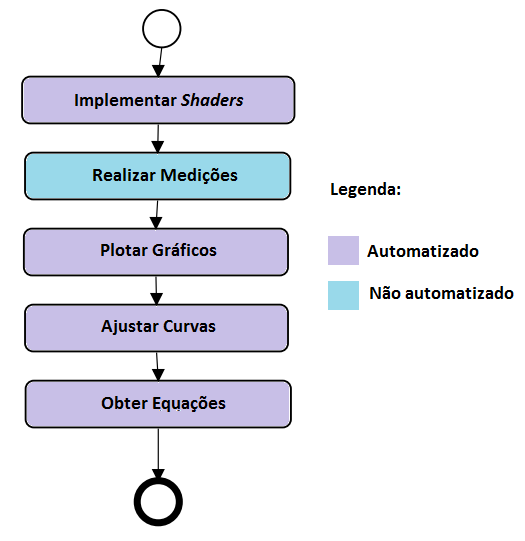
\includegraphics[keepaspectratio=true,scale=0.5]{figuras/processo.png}
	\caption{Processo da Análise de Complexidade Algorítmica.}
	\label{processo}
	\end{figure}

	\begin{figure}[ht]
	\centering
		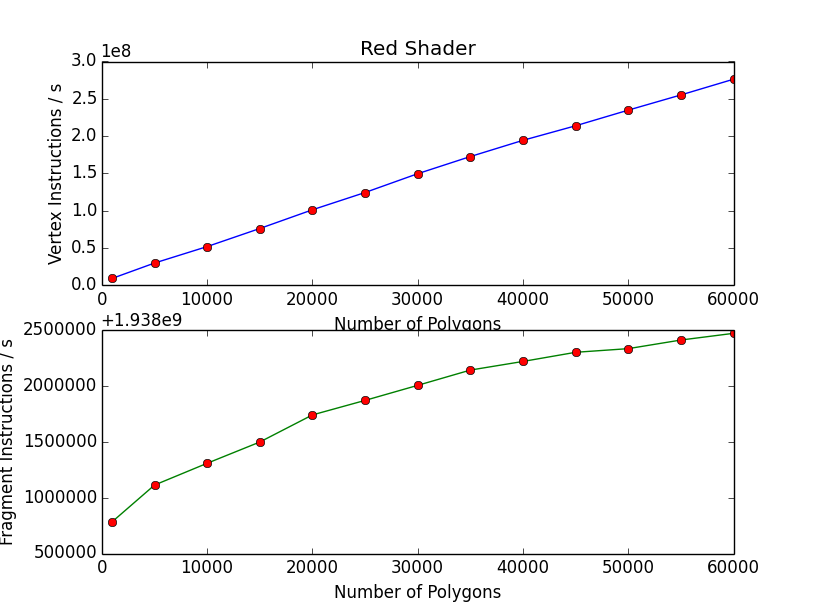
\includegraphics[keepaspectratio=true,scale=0.55]{figuras/red.png}
	\caption{Gráficos: \textit{Red Shader}, \textit{Toon shader}, \textit{Gouraud Shader},  \textit{Phong Shader} e  \textit{Flat Shader}}
	\label{plotred}
	\end{figure}

 
	\begin{figure}[ht]
	\centering
		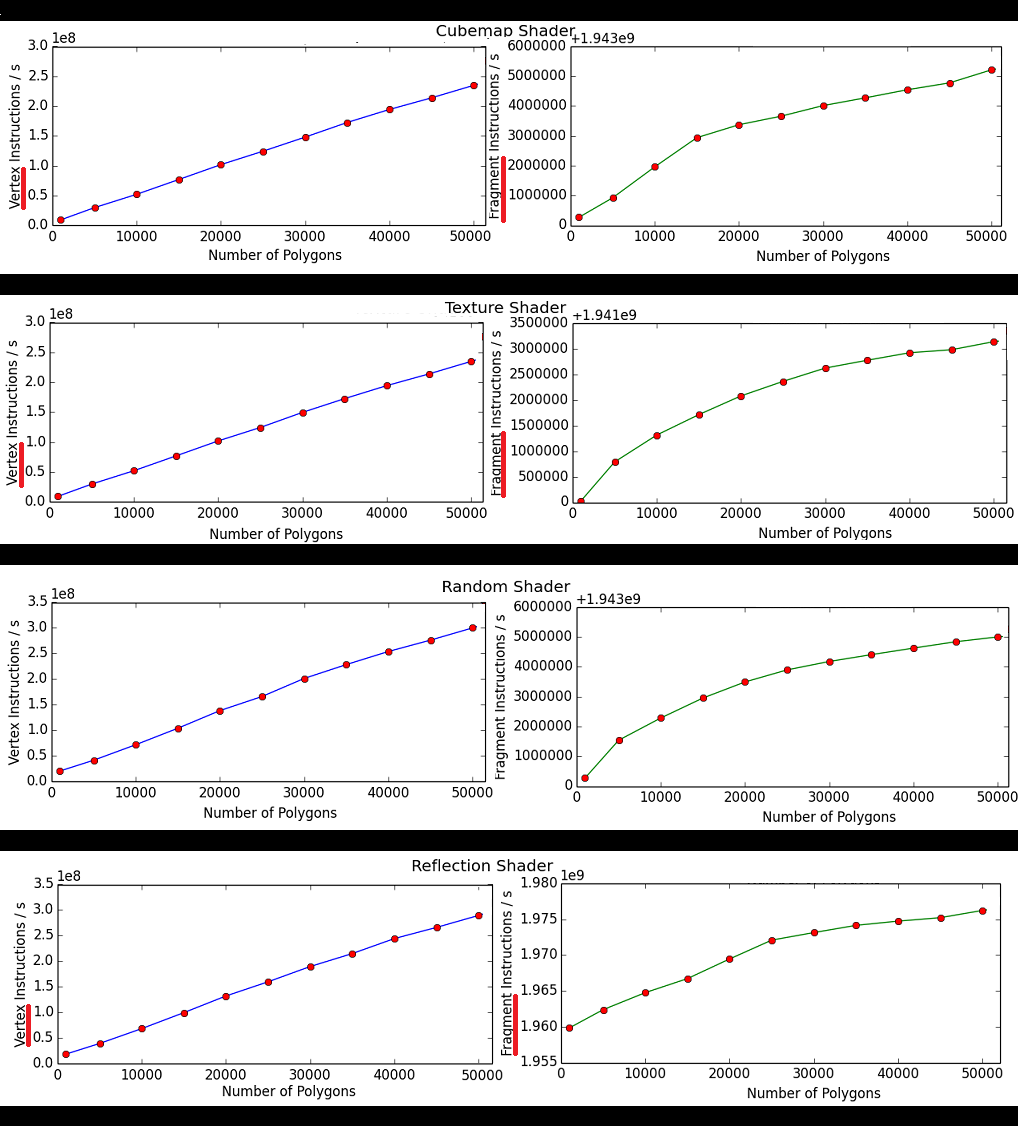
\includegraphics[keepaspectratio=true,scale=0.55]{figuras/cubeplot.png}
	\caption{Gráficos: \textit{Cubemap Shader}, \textit{Texture Shader}, \textit{Random Shader}, \textit{Reflection Shader}}
	\label{plotrefl}
	\end{figure}


	\begin{figure}[ht]
	\centering
		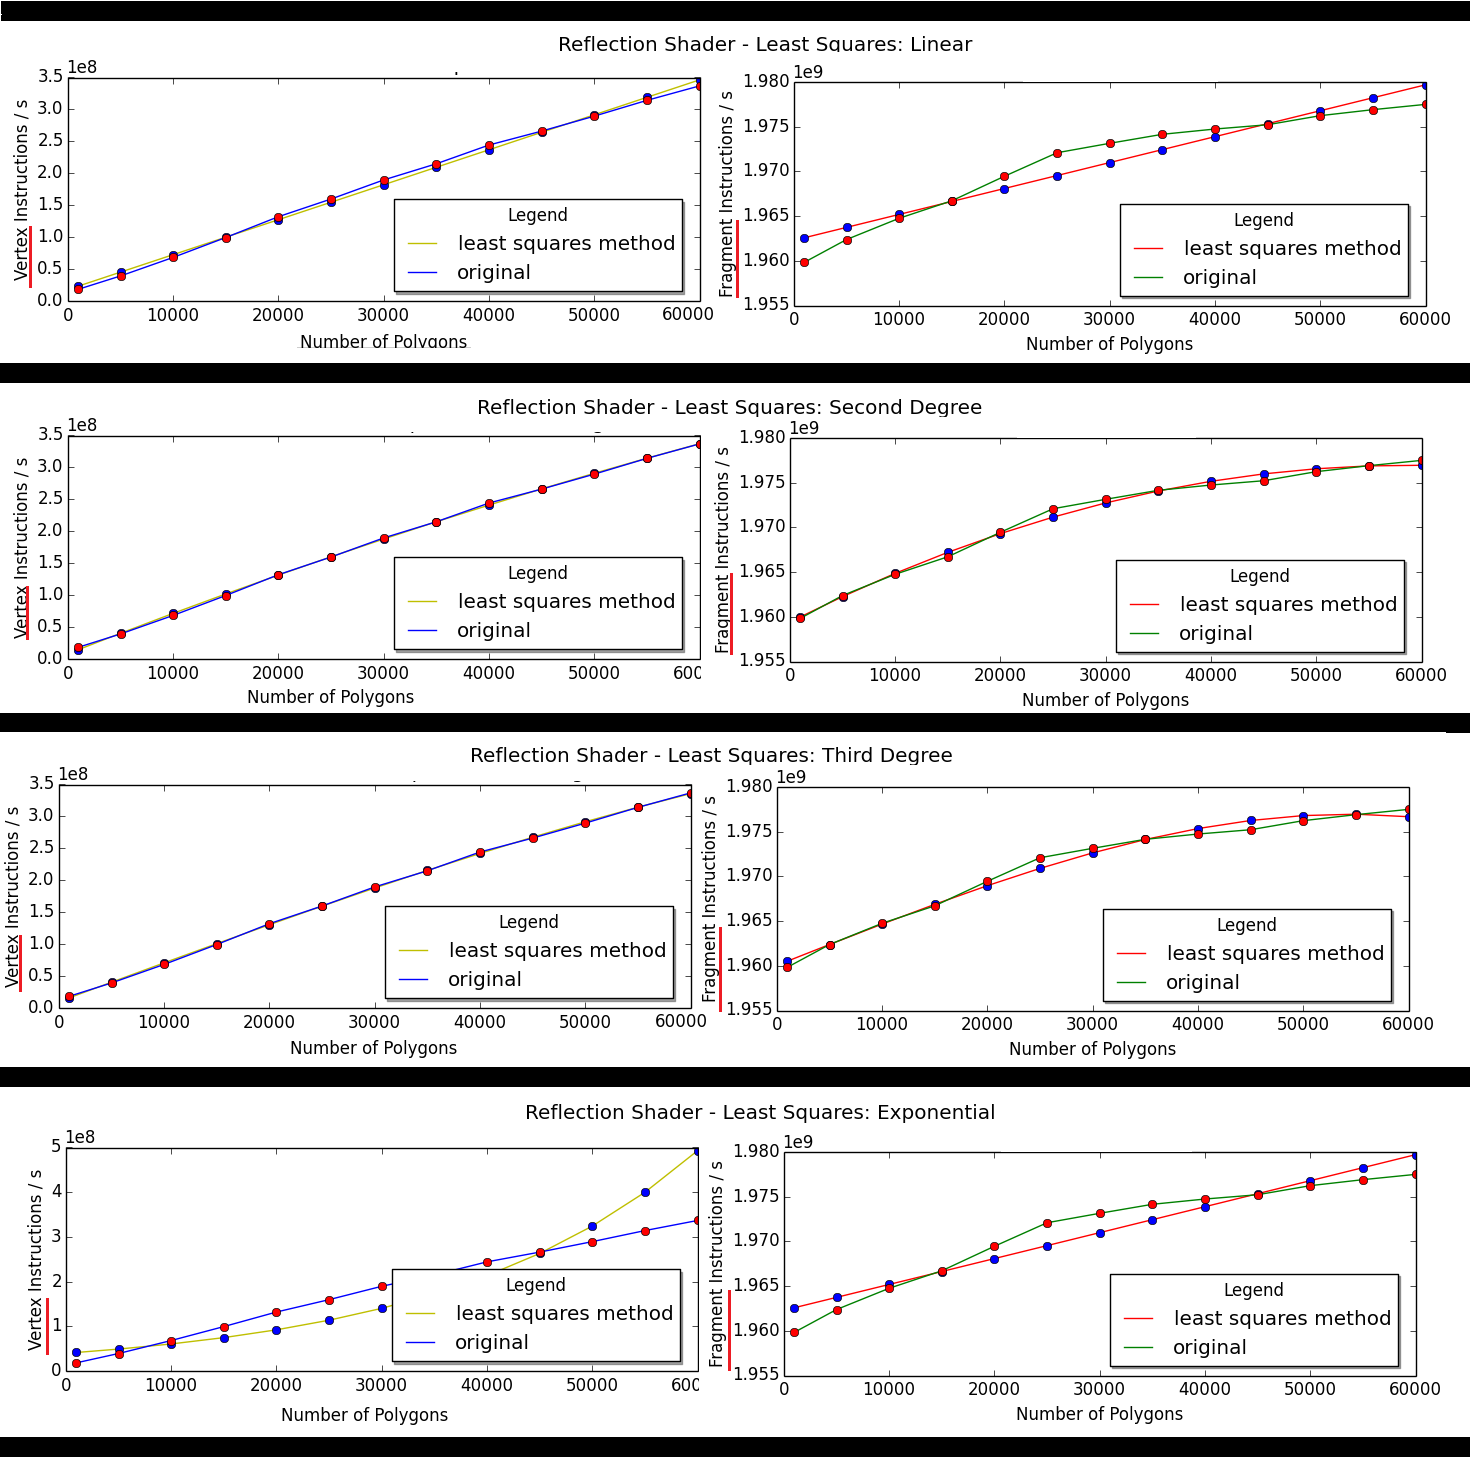
\includegraphics[keepaspectratio=true,scale=0.4]{figuras/reflectionlinear.png}
	\caption{Ajustes linear, segundo, terceiro graus e exponencial para cada tipo de \textit{shader}}
	\label{linear}
	\end{figure}	

	\begin{figure}[ht]
	\centering
		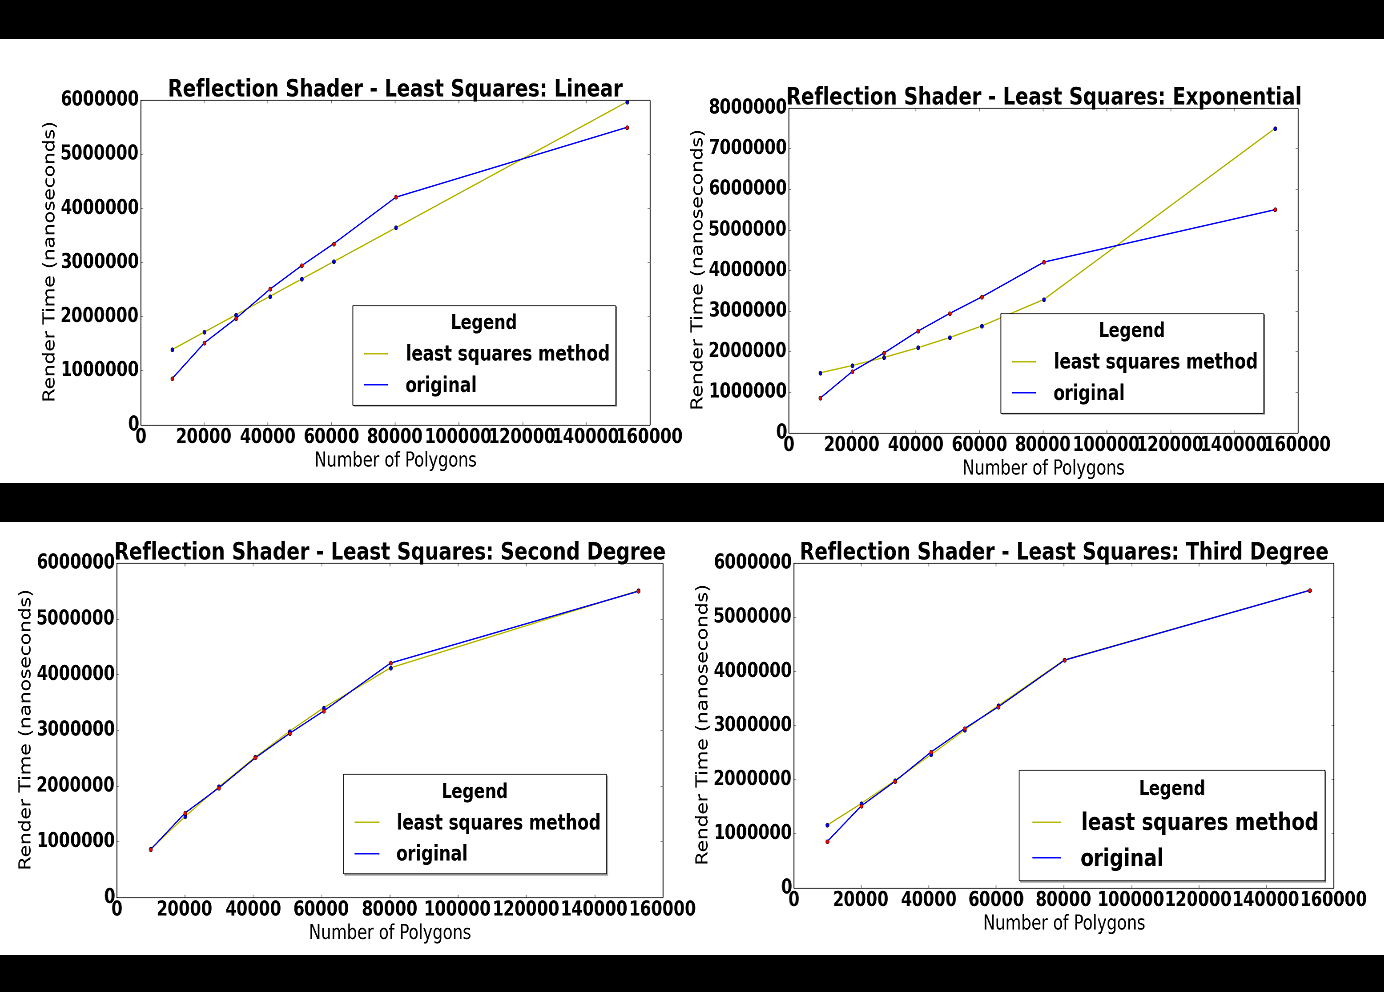
\includegraphics[keepaspectratio=true,scale=0.4]{figuras/minquad_render_time.png}
	\caption{Ajustes linear, segundo, terceiro graus e exponencial para processo de renderização}
	\label{linear}
	\end{figure}	
	
